\documentclass[UserManual.tex]{subfiles}
\begin{document}
\setcounter{section}{1}

\section{Installation and Getting Started}\label{sec:installation}

\subsection{Prerequisites}
{\it Smooth Emulator} software should run on UNIX, Mac OS or Linux, but is not supported for Windows OS. {\it Smooth Emulator} is largely  written in C++. In addition to a C++ compiler, the user needs the following software installed.

\begin{itemize}
    \item git
    \item CMake
    \item Eigen3 (Linear Algebra Package)
    \item Python/Matplotlib (only for generating plots in the MCMC procedure)
\end{itemize}

CMake is an open-source, cross-platform build system that helps automate the process of compiling and linking for software projects. Hopefully, CMake will perform the needed gymnastics to find the Eigen3 installation. To install CMake, either visit the CMake website (https://cmake.org/), or use the system's package manager for the specific system. For example, on Mac OS, if one uses {\it homebrew} as a package manager, the command is
{\tt 
\begin{verbatim} % brew install cmake\end{verbatim}
}

Eigen is a C++ template library for vector and matrix math, i.e. linear algebra. The user can visit the Eigen website (\url{https://eigen.tuxfamily.org/dox/}), or use their system's package manager. For example on Mac OS with {\it homebrew},
{\tt 
\begin{verbatim} % brew install eigen\end{verbatim}
}

\subsection{Downloading the Repository and Setting the GITHOME\_BAND\_SMOOTH Environment Variable}

The software requires downloading the BAND framework software repository into some directory. Should that be in the User's home directory, the User might enter
{\tt 
\begin{verbatim}
    /Users/CarlosSmith% git clone https://github.com/bandframework/bandframework.git
\end{verbatim}
}
The User needs to set an environmental variable, {\tt GITHOME\_BAND\_SMOOTH}, to the full path of the directory where the software is located, e.g. 
{\tt
\begin{verbatim}
    % export GITHOME_BAND_SMOOTH="/Users/CarlosSmith/bandframework/software/SmoothEmulator"
\end{verbatim}
}
It is recommended to copy this command into the user's {\tt .bashrc} (or equivalent) file to avoid re-defining it each time one needs to recompile. Throughout the manual the phrase {\tt GITHOME\_BAND\_SMOOTH} will refer to this directory. 

The User needs to create a project directory from which the User would perform most projects. This is easiest accomplished by copying a template from the {\it Smooth} distribution,
{\tt
\begin{verbatim}
    % cp -r GITHOME_BAND_SMOOTH/templates/myproject MY_PROJECT
\end{verbatim}
}
Hence forth, {\tt MY\_PROJECT} will refer to the directory, including the path, from which the User will perform most of the analysis. The User may wish to have several such directories. These directories should be outside the main distribution, i.e. outside the {\tt bandframework/} path. 

Although the main source code, include files and libraries are all located in the software directory, the main programs and executables are not. The motivation for this decision is to allow the User to easily modify their own versions of the main programs. These tend to be very short programs. For that reason their is a separate directory to store the main programs and their executables. The User can easily set this up by copying a template directory,
{\tt 
\begin{verbatim}
    % cp -r GITHOME_BAND_SMOOTH/templates/mylocal MY_LOCAL
\end{verbatim}
}
Here {\tt MY\_LOCAL} will hence forth refer to the path of this directory. This directory should be outside the main distribution, i.e. outside the {\tt bandframework/} path. 

For the remainder of this manual, {\tt GITHOME\_BAND\_SMOOTH}, {\tt MY\_LOCAL} and {\tt MY\_PROJECT} will be used to denote the location of these directories.

\subsection{Directory and File Structure}

\begin{figure}
\centerline{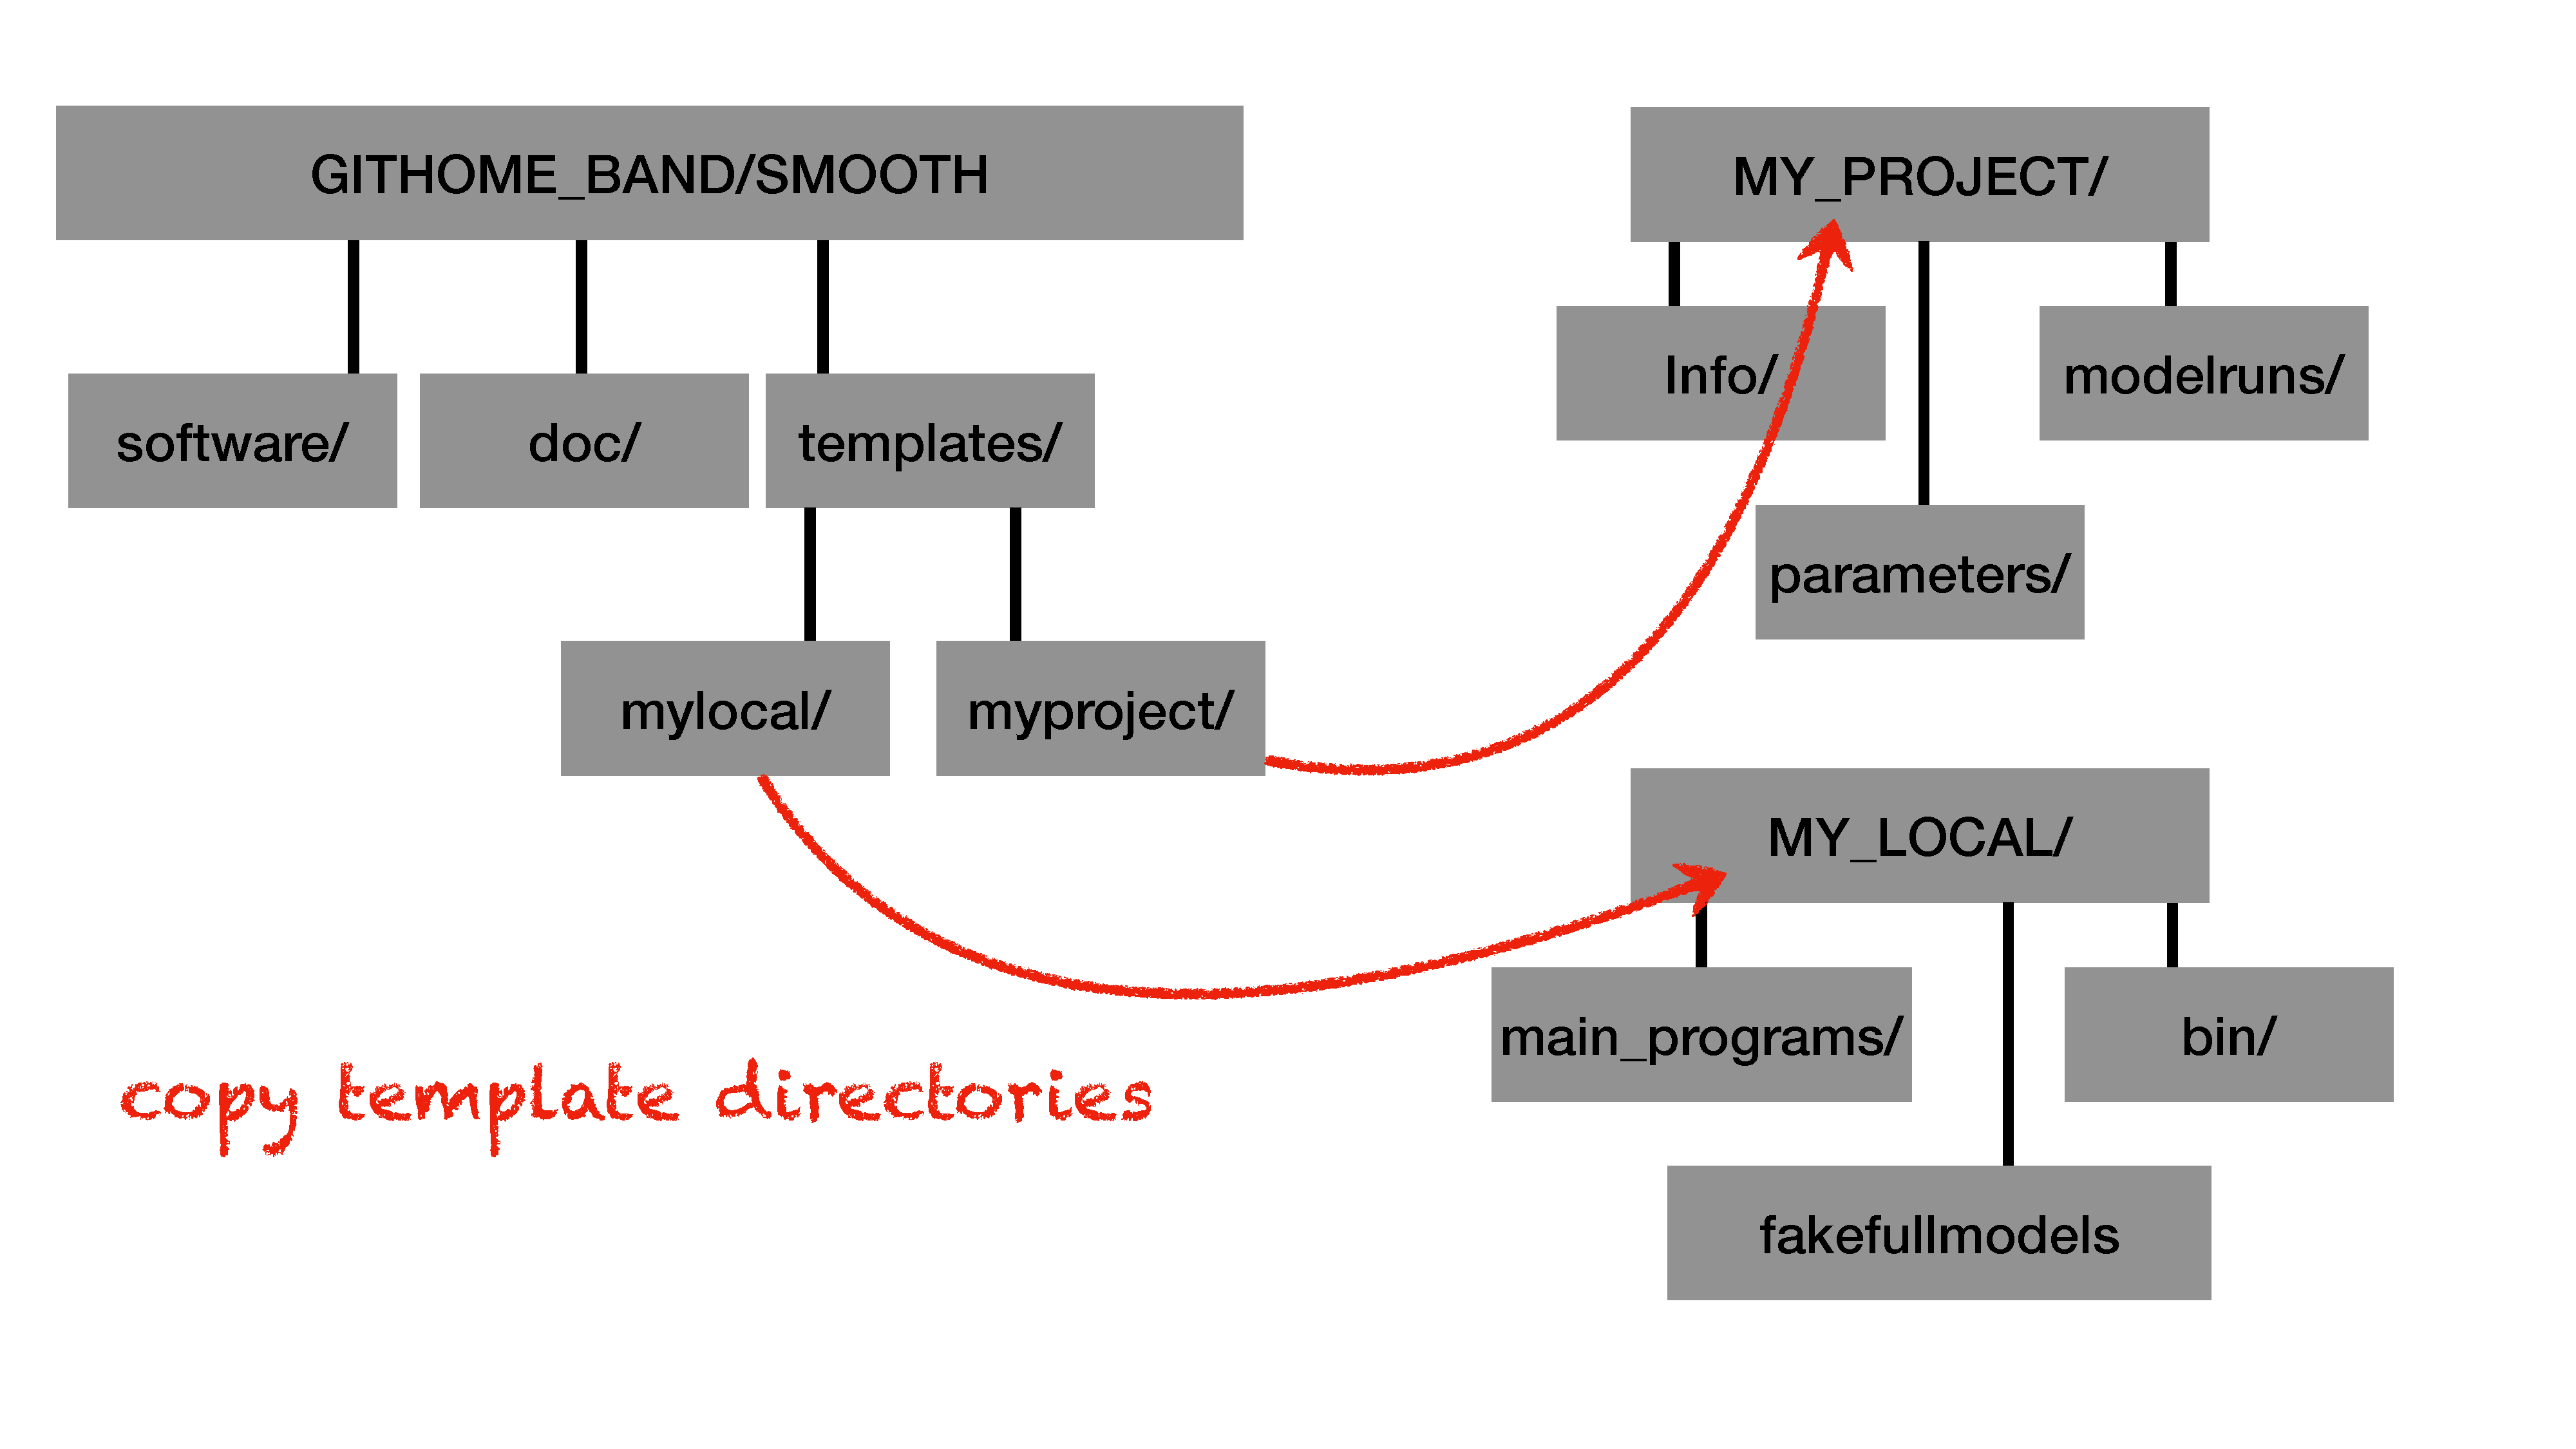
\includegraphics[width = 0.95\textwidth]{directorystructure}}
\caption{{\bf The directory structure}: The User clones two repositories into some location, which will be referred to as {\tt GITHOME\_BAND}. The User can then copy two template directories into the User's choices of locations outside the path of the BAND repositories. The name of those two directories will be referred to as {\tt MY\_LOCAL}, which will contain the main programs and executables, and {\tt MY\_PROJECT} which contains the data files related to a given project. The programs are designed to be run from within the {\tt MY\_PROJECT/} directory.}
\end{figure}

Once compiled, the libraries in the {\tt commonutils/} directory are used for a variety of tasks. These libaries are not particularly designed for {\it Smooth Emulator} or {\it Simplex Sampler}. The {\tt SmoothEmulator/} directory contains codes that are used to create libraries specific to the sampler and emulator. The executables are stored in {\tt MY\_LOCAL/bin}. The short main program source files are located in {\tt MY\_LOCAL/main\_programs/}. It is not envisioned that the User would edit files in the {\tt SmoothEmulator/software/} directory, but that the User may well wish to create custom versions of the short main programs in {\tt MY\_LOCAL/main\_programs/}. The main programs are compiled using the CMake files in {\tt MY\_LOCAL/build/}. The User may find it convenient to add {\tt MY\_LOCAL/bin/} to their path.

\subsection{Compiling Libraries }

First, change into software directories, then create the makefiles with cmake, then compile them.
{\tt 
\begin{verbatim}
    % cd GITHOME_BAND_SMOOTH/software
    GITHOME_BAND_SMOOTH/software% cmake .
    GITHOME_BAND_SMOOTH/software% make
\end{verbatim}
}
There seems to be a common problem that {\tt cmake} misreports the path the {\tt Eigen} installation. If the User should get an error stating that the Eigen header files cannot be found, the User can set one of the following environmental variables,
{\tt 
\begin{verbatim}
    % export EIGEN3_INCLUDE_DIR=/usr/local/include/eigen3
\end{verbatim}
}
The final arguments may need to be changed depending on the User's location of the packages.

At this point all the libraries are built, but this does not include the main programs. The main programs are short, and are located in a separate location, as they are meant to serve as examples which the User might copy and edit at will.

Finally, compile the main programs. Below, this illustrates how to build the programs used for generating training points with Simplex and for tuning the emulator with Smoothy:
{\tt
\begin{verbatim}
    % cd MY_LOCAL/build
    MY_LOCAL/build% cmake .
    MY_LOCAL/build% make simplex
    MY_LOCAL/build% make smoothy_tune
    .
    .
\end{verbatim}
}
Other source codes for main programs can be found in {\tt MY\_LOCAL/main\_programs/}. If you build your own main programs (probably using these as examples), you can edit the {\tt CMakeList.txt} file in {\tt GITHOME\_BAND\_SMOOTH/local/build}, using the existing entries as an example. The executables should appear in {\tt MY\_LOCAL/bin/}. 

\subsection{The Project Directory}

Within {\tt MY\_PROJECT/} there are three sub-directories (assuming it was created from the template). The first is {\tt MY\_PROJECT/Info/}. Information about the model parameters, and their priors is stored in {\tt MY\_PROJECT/Info/modelpar\_info.txt}, and information about the observables is stored in {\tt MY\_PROJECT/observable\_info.txt}. The {\tt MY\_PROJECT/parameters} directory stores user-defined parameter files used by {\it Simplex Sampler}, {\tt MY\_PROJECT/parameters/simplex\_parameters.txt}, and by {\it Smooth Emulator} {\tt MY\_PROJECT/parameters/emulator\_parameters.txt}. The {\tt MY\_PROJECT/modelruns} directory will store information for each full-model run. The directories {\tt  MY\_PROJECT/modelruns/run0/}, {\tt  MY\_PROJECT/modelruns/run1/}, $\cdots$, have files describing the model parameters for each run, along with the output required by the emulator for each specific full-model run. For example, the {\tt  MY\_PROJECT/modelruns/run1/} directory has the files {\tt mod\_parameters.txt} and {\tt obs.txt}. The first file stores the model parameter values for that particular training run. The User then runs their full model based on those parameters and stores the corresponding observables in {\tt obs.txt}. The User may generate the {\tt mod\_parameters.txt} files using {\it Simplex Sampler}, or the user might generate them according to some other prescription. Once the User has then generated the {\tt obs.txt} files, {\it Smooth Emulator} can then build and tune the emulator.

\end{document}
